\chapter{Introducción}
El presente trabajo de tesis está dedicado al diseño, construcción e implementación de un sistema automatizado para la realización de estudios de espectroscopia, utilizando un monocromador como sistema para descomponer la luz  en sus diferentes longitudes de onda y un tubo fotomultiplicador (PMT) para medir la intensidad luminosa de cada una.

La espectroscopia óptica es una herramienta utilizada para el estudio de la luz absorbida o emitida por la materia, El intervalo del espectro electromagnético que se estudiará parte de los 200 nm hasta los 650 nm (Ultravioleta medio, ultravioleta cercano y luz visible), ver figura \ref{fig:espectrovisible}.
\begin{figure}[h!]%figura 1
	\centering
	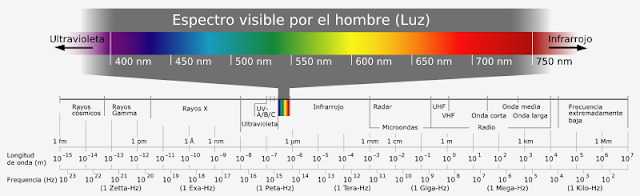
\includegraphics[width=1\linewidth]{Imagenes/espectro_visible}
	\caption{Espectro electromagnético, enfatizando el espectro visible para el ojo humano \cite{espectroOjo}.}
	\label{fig:espectrovisible}
\end{figure}

\section{Espectro electromagnético.}
Se denomina espectro electromagnético a la distribución energética del conjunto de las ondas electromagnéticas. Referido a un objeto se le llama espectro de la radiación electromagnética que emite o absorbe el mismo y que se relaciona con su composición. Dicha radiación nos brinda información sobre la materia y sirve para identificar las sustancias, el espectro es único para cada sustancia de manera análoga a una huella dactilar. 
\begin{figure}[h!] %figura 2
	\centering
	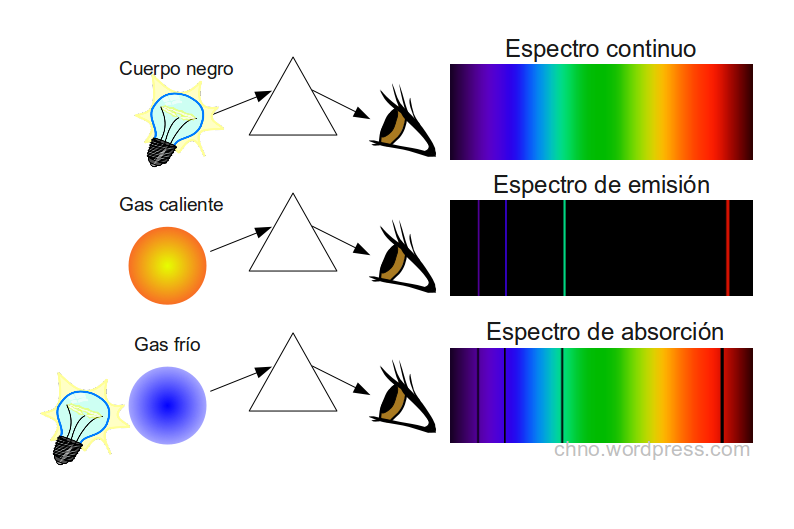
\includegraphics[width=1\linewidth]{Imagenes/espectros_absorcion_y_emision}
	\caption{Tipos de espectros. \cite{FisicaCh}}
	\label{fig:esq_espectro01}
\end{figure}

En la figura \ref{fig:esq_espectro01} se observan diferentes espectros y cómo se producen estos, donde el primero, es el espectro continuo o de cuerpo negro, en el cuál se observa una banda continua. Es emitido por cualquier objeto caliente, el espectro solar es un ejemplo de este. El espectro de emisión es generado cuando los átomos y moléculas en un gas caliente emiten una radiación en ciertas longitudes de onda. Por otra parte el espectro de absorción se observa cuando el mismo gas, recibe radiación electromagnética, este gas absorbería ciertas longitudes de onda. Se observa que las líneas emitidas son las mismas que las que no se presentan cuando absorbe. Cumpliendo con esto la ley de Kirchhoff de la radiación térmica: \emph{si un cuerpo (o superficie) está en equilibrio termodinámico con su entorno, su emisividad es igual a su absortividad} $\alpha = \epsilon$.

\subsection{Intervalo energético del espectro.}
El espectro electromagnético cubre longitudes de onda muy variadas. Existen frecuencias desde 30 HZ y menores que son relevantes en el estudio de ciertas nebulosas. Por otro lado se conocen frecuencias cercanas a los  $2.9*10^{27}$ Hz, que han sido detectadas provenientes de rayos cósmicos.
La energía de una onda electromagnética es determinada por su longitud de onda, la cual tiene una frecuencia asociada, y una energía de fotón E. La relación es la siguiente.
$c = f\lambda$, o, $\lambda = c/f$. La energía de un fotón está dada por la siguiente ecuación.
\begin{equation}
E = hf =h\cdot \frac{c}{\lambda}
\label{equa:intcuad}
\end{equation}
\begin{itemize}
	\item $h$ constante de Planck, $h \approx 6.626069\times 10^{34} J\cdot s$.
	\item $\lambda$ longitud de onda en ($nm$).
	\item $f$ frecuencia de la luz ($Hz$).
	\item c velocidad de la luz en el vacio $c = \frac{1}{\sqrt{\mu_0\epsilon_0}}$, $c = 299,792,458 m/s$
	\subitem $\mu_0$ permeabilidad en el vacío $\mu_0 = 4\pi\times10^{-7} N\cdot A^{-2}$
	\subitem $\epsilon_0$ es la permitividad en el vacío $\epsilon_0 = 8.85418\times10^{12} C^2/N\cdot m^2$
	
\end{itemize}
Podemos reescribir la ecuación \ref{equa:intcuad}, expresando la energía $E$ en $eV$, la longitud de onda ya en nanómetros ($nm$) y las constantes $h$ y $c$, $1eV = 1.6\times 10^{-19} J$
\begin{equation}
E(ev)\approx \frac{1240}{\lambda}
\label{equa:intcuad2}
\end{equation}
De modo que para un fotón de longitud de onda igual a 200nm se tiene una energía de 6.2eV mientras que para uno de 700nm la energía será de 1.77eV.
$$E_{200}\approx \frac{1240}{200}=6.2eV $$
$$E_{700}\approx \frac{1240}{700}=1.77eV $$
De la ecuación \ref{equa:intcuad2} podemos observar la energía es inversamente proporcional a la longitud de onda, a longitudes de onda menores tendremos mayor energía, y a mayor longitud de onda menos energía.
Las ondas electromagnéticas se clasifican en: rayos-$\gamma$, rayos-x, ultravioleta, luz visible, infrarrojos, microondas y ondas de radio.

\subsection{Región visible}
El intervalo de luz visible va desde los 400nm hasta los 700nm aproximadamente, se le llama así a esta región por ser el intervalo donde el ojo humano tiene sensibilidad, ver figura \ref{fig:ojohumano}. La máxima sensibilidad del ojo humano se encuentra a los 555nm (verde), la respuesta espectral del ojo humano fue establecida por la CIE, Commission internationale de l'éclairage \cite{CIE1924}.

En la tabla \ref{tabla:ojo},  se observan los intervalos en longitud de onda para los colores que componen la luz blanca.
Newton fue el primero en darse cuenta que la luz blanca está compuesta de todos los colores del espectro visible.
\begin{figure}
	\centering
	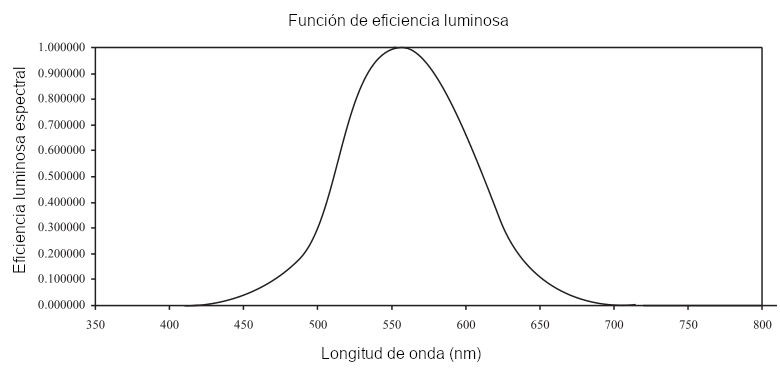
\includegraphics[width=0.8\linewidth]{Imagenes/SpectralL}
	\caption{Sensibilidad del ojo humano ante el espectro electromagnético, \cite{CRC2016}, \cite{inproceedings}}
	\label{fig:ojohumano}
\end{figure}

\begin{table}
\centering

\caption{Intervalos de longitud de onda en el vacío para los distintos colores. \cite{Bruno2005}}
\begin{tabular}{|c|c|}
	\hline 
	Color & $\lambda$ Longitud de onda ($nm$) \\ 
	\hline 
	Violeta & 380-450 \\ 
	\hline 
	Azul & 450-495  \\ 
	\hline 
	Verde & 495-570  \\ 
	\hline 
	Amarillo & 570-590 \\ 
	\hline 
	Naranja & 590-620 \\ 
	\hline 
	Rojo & 620-750 \\ 
	\hline 
\end{tabular} 
\label{tabla:ojo}		
\end{table}


\subsection{Ultravioleta}
La luz ultravioleta es el intervalo del espectro electromagnético que va desde los 10nm hasta los 400nm, se puede dividir en varios intervalos definidos por la \textbf{ISO 21348} \cite{Solar}. En la tabla \ref{tabla:UV} se muestran las subcategorías para el ultravioleta. En este trabajo utilizaremos las subcategorías NUV y MUV (200-400 $nm$). 
\begin{table}
	\centering
	\caption{ISO 21348 sección de subcategorías del ultravioleta. \cite{Solar}} 
	\label{tabla:UV}
	\begin{tabular}{|c c c|}
		\hline
		Subcategoria UV & Intervalo en \textbf{$nm$} & Descripción. \\
		\hline
		UV & 10$\leq\lambda\leq$400 & Ultravioleta \\
		\hline
		\hline
		UVA & 315$\leq\lambda\leq$400 & Ultravioleta A\\
		UVB & 280$\leq\lambda\leq$315 & Ultravioleta B\\
		UVC & 100$\leq\lambda\leq$280 & Ultravioleta C\\
		\hline
		\hline
		NUV & 300$\leq\lambda\leq$400 & Ultravioleta cercano\\
		MUV & 200$\leq\lambda\leq$300 & Ultravioleta medio\\
		FUV & 122$\leq\lambda\leq$200 & Ultravioleta lejano\\
		H-Lyman-$\alpha$ & 121$\leq\lambda\leq$122 &  linea Lyman alfa\\
		\hline\hline
		VUV & 10$\leq\lambda\leq$200 & Ultravioleta de vacío\\
		EUV & 10$\leq\lambda\leq$121 & Ultravioleta extremo.\\
		\hline
	\end{tabular}
\end{table}

\section{Espectrometría.}
La interacción de la radiación electromagnética con la materia se puede describir con una representación gráfica de la distribución de intensidad de la radiación electromagnética, emitida o absorbida, por una sustancia, en función de su longitud de onda. Al analizar la radiación emitida o absorbida por la materia, se pueden identificar sustancias que la componen. 


\section{Espectrómetro}
El espectrómetro óptico es un dispositivo utilizado para analizar la luz, para esto, el espectrómetro descompone la luz a estudiar en sus diferentes longitudes de onda que la componen, y mide la intensidad luminosa en cada una de estas longitudes de onda. Con lo cual obtendremos una gráfica de la intensidad contra la longitud de onda. Fig. \ref{fig:espectrosol} \cite{B&WTek2016}. 

\subsection{Funcionamiento del espectrómetro.}
El funcionamiento básico del espectrómetro es descomponer la luz en sus componentes espectrales, medir la intensidad de la señal en función de la longitud de onda, y graficar las intensidades medidas en relación con la longitud de onda. 
%\begin{enumerate}[a]
%	\item Ranura de entrada o \textsl{slit}.
%	\item Espejo colimador.
%	\item Red de difracción.
%	\item Detector
%\end{enumerate}
\begin{figure}[h!]
	\centering
	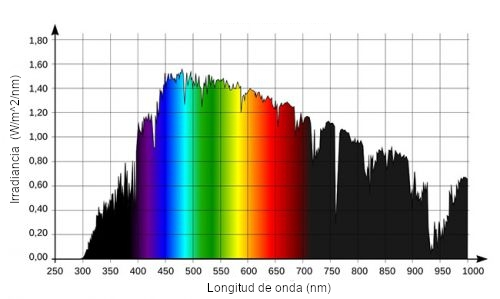
\includegraphics[width=0.9\linewidth,height=5cm]{Imagenes/espectroSOL}
	\caption{Espectro continuo, luz solar \cite{SolarLight}.}
	\label{fig:espectrosol}
\end{figure}

El primer paso es introducir la luz al espectrómetro, la luz entra por medio de una fibra óptica, pasando por una pequeña apertura, \textbf{la ranura de entrada}, ver la figura \ref{fig:esquematicoespectrometro}(a). Aquí la luz diverge, esta luz es colimada utilizando un \textbf{espejo cóncavo} figura \ref{fig:esquematicoespectrometro}(b) y reflejada hacia la \textbf{red de difracción} figura \ref{fig:esquematicoespectrometro}(c). Aquí ocurre el fenómeno de difracción separando la luz en sus diferentes componentes espectrales, cada componente espectral se refleja en un ángulo diferente, las cuales son enfocadas por un segundo \textbf{espejo cóncavo} figura \ref{fig:esquematicoespectrometro}(d), al final son proyectadas en el \textbf{detector} figura \ref{fig:esquematicoespectrometro}(e). La señal luminosa es entonces convertida a una señal eléctrica. Con base en la dispersión lineal
de la red de difracción y los pixeles en el detector, el software obtiene la relación en
longitud de onda, y así se obtiene un espectro de intensidad en función de la longitud de onda.

\begin{figure}[h]
	\centering
	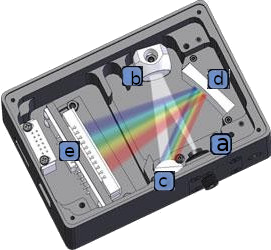
\includegraphics[width=0.55\linewidth]{Imagenes/Espectrometro}
	\caption[Esquema de un espectrómetro.]{Esquemático de un espectrómetro. Se aprecia como la luz es colimada, refractada y enfocada al sensor CCD \cite{BWTEK}}
	\label{fig:esquematicoespectrometro}
\end{figure}

\subsubsection{Ranura de entrada.}
La ranura de entrada o \textit{slit} de entrada, es la entrada de luz al espectrómetro, aquí es donde se define la \textit{cantidad de luz, flujo de fotones}, que entrara en el espectrómetro, fig. \ref{fig:colimarluz} punto (a).
El \textit{slit} es de suma importancia para determinar la resolución óptica del sistema, Normalmente los espectrómetros cuentan con diferentes aperturas de esta ranuras, que van desde los 5$\mu m$ hasta los 200$\mu m$, siendo seis las más comunes: 5$\mu m$, 10$\mu m$, 20$\mu m$, 25$\mu m$, 50$\mu m$, 100$\mu m$ o 200$\mu m$, \cite{Oceana}.

\subsubsection{Espejo colimador.}
Se encarga de hacer que los haces que han pasado por la ranura de entrada sean colimados. Utilizando un espejo cóncavo y teniendo el foco del espejo en la ranura de entrada, hace que todos los haces sean reflejados de forma paralela entre ellos, luz colimada, fig. \ref{fig:colimarluz}, espejo (C). 

\begin{figure}[h]
	\centering
	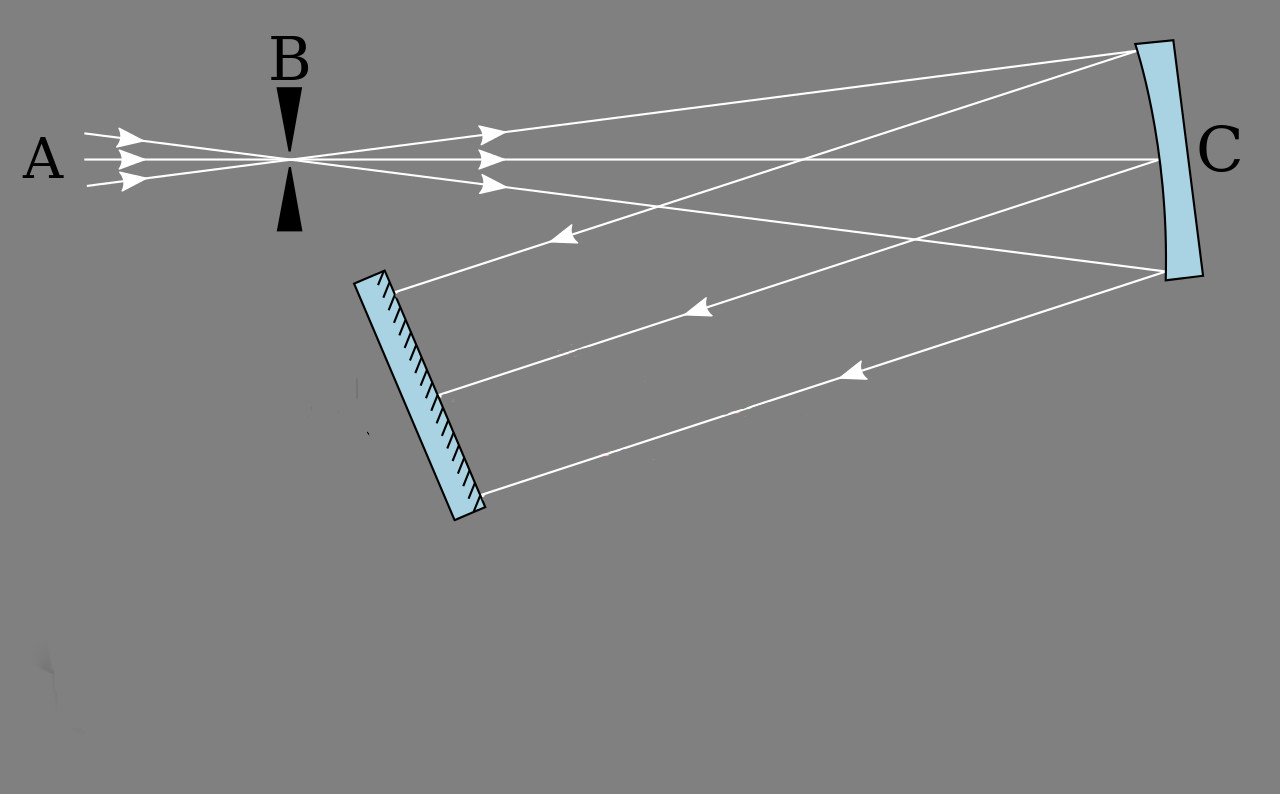
\includegraphics[width=0.6\linewidth]{Imagenes/ColimarLuz}
	\caption{Diagrama óptico de los haces a la entrada del monocromador y colimados hacia la red de difracción. \cite{Czerny-Turney-Conf}}
	\label{fig:colimarluz}
\end{figure}

\subsubsection{Red de difracción.}
Se encarga de descomponer la luz en sus diferentes longitudes de onda, por lo tanto, la red de difracción determina el intervalo de longitudes de onda y en parte la resolución óptica del sistema. 
Existen dos tipos de redes de difracción dadas por la forma en la que son construidas.
\begin{itemize}
	\item Red de difracción regladas: Es hecha con una herramienta con punta de diamante que realiza cortes en un revestimiento que es una capa reflejante sobre un vidrio.
	\item Red de difracción holográfica: A diferencia de la anterior, tiene como herramienta el uso de una litografía por interferencia láser, este proceso permite líneas más cercanas, con menos errores.
\end{itemize}

A su vez las redes de difracción pueden ser de transmisión o de reflexión, Y de forma cóncava o plana. En la figura \ref{fig:redes}(a) se muestra como la luz reflejada es difractada. Mientras que en \ref{fig:redes}(b) la difracción ocurre cuando la luz pasa a través de una rejilla. La figura \ref{fig:redes}(c) y (d) son ejemplos de redes, (c) red plana y (d) red cóncava.

\begin{figure}[h]
	\centering
	\subfigure[Red por reflexión]{	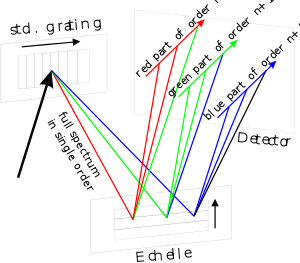
\includegraphics[width=0.4\linewidth, height=3cm]{Imagenes/300px-Echelle_Principle}}
	\subfigure[Red por transmisión]{	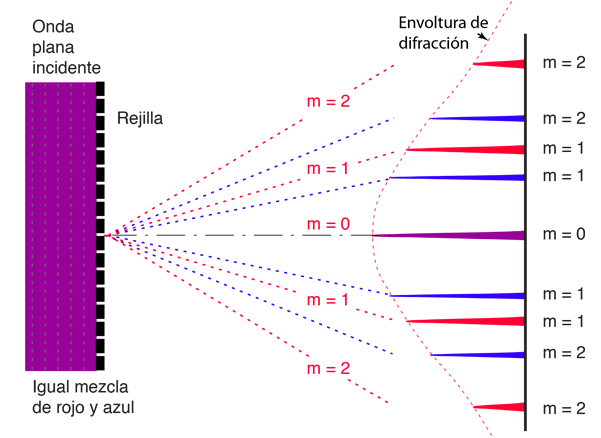
\includegraphics[width=0.4\linewidth,height=3cm]{Imagenes/DiffGrat}}
	\subfigure[Red de difracción plana]{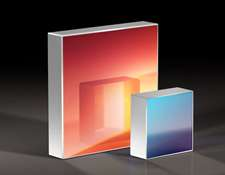
\includegraphics[width=0.4\linewidth,height=3cm]{Imagenes/rejillaPlana}}
	\subfigure[Red de difracción cóncava]{	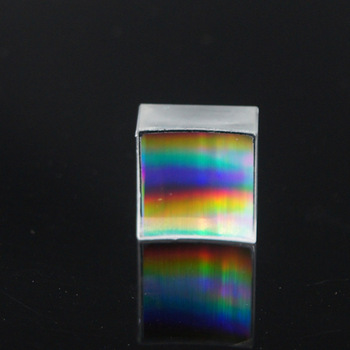
\includegraphics[width=0.4\linewidth,height=3cm]{Imagenes/Spectral-components-Concave-Holographic-Gratings-for-Monochromator}}
	\caption{Redes de difracción, las más comunes son las redes de difracción planas y cóncavas, aún que pueden tener otras formas, como convexa o toroidal \cite{ThorLabs}.}
	\label{fig:redes}
\end{figure}

\subparagraph{Redes de difracción de reflexión.}
La luz incidente en la superficie de estas redes es reflejada a diferentes ángulos, los cuales dependen de la longitud de onda. Con lo cual se puede seleccionar un intervalo espectral. Para calcular este ángulo se usa la ecuación \ref{equa:RedDifra}. Donde \textit{m} es el número de orden, $\lambda$ es la longitud de onda, \textit{d} es la distancia entre líneas contiguas en la red de difracción, $\alpha$ es el ángulo incidente, y $\beta$ el ángulo al que es reflejado, véase figura \ref{fig:reflexion}.
\begin{equation}
	m\lambda = d(\sin\alpha + \sin\beta)
	\label{equa:RedDifra}
\end{equation}
\begin{figure}[h]
	\centering
	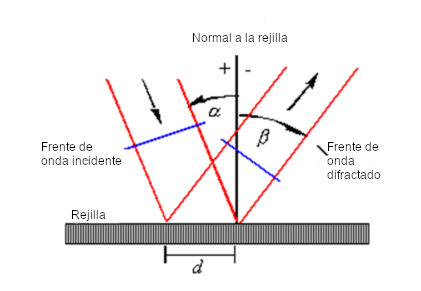
\includegraphics[width=0.6\linewidth]{Imagenes/reflexion}
	\caption{Diagrama de la incidencia y reflexión del haz sobre una red de difracción. $\alpha$ es el ángulo incidente, $\beta$ el reflejado, $d$  es la distancia entre cada línea en la red de difracción, $\lambda$ la longitud de onda. \cite{Excel2000}}
	\label{fig:reflexion}
\end{figure}


\subparagraph{Redes de difracción de transmisión.}
Cuando son de transmisión $\alpha$ es igual a cero ya que la luz incide perpendicular al plano de la red. Sustituyendo ese valor en la ecuación \ref{equa:RedDifra}, se simplifica a
\begin{equation}
m\lambda = d\sin\beta
\label{equa:difra}
\end{equation}
\subsubsection{Detector.}
En los espectrómetros actuales frecuentemente el sensor que se utiliza es el CCD, \textit{charge-coupled device}, con este sensor, cada uno de sus pixeles representa una porción del espectro electromagnético. Así al incidir la luz reflejada por la red de difracción se obtiene un espectro inmediato el cual puede ser visualizado en una computadora por medio de un software.

\section{Monocromador}
El monocromador es un dispositivo utilizado para separar la luz en sus diferentes componentes a diferencia de los espectrómetros actuales en los cuales se pueden medir u observar un ancho de banda (todo el espectro visible). En el monocromador, como su nombre lo dice, \textit{mono}, uno, y \textit{chroma} color, nos dice que a la salida del monocromador solo obtendremos una longitud de onda, de todas las que esta compuestas la luz.
El monocromador permite hacer barridos, estos barridos no es otra cosa que modificar el
ángulo de incidencia de la luz en la red de difracción. Con lo que se puede ir visualizando a la salida del monocromador, las diferentes longitudes de onda que componen la luz a estudiar. El monocromador, ver figura \ref{fig:1280px-czerny-turnermonochromator}, es similar en configuración a un espectrómetro, la diferencia radica en que después de la rejilla de difracción hay un espejo que se encarga de enfocar las longitudes de onda a una ranura de salida, \textit{slit}, que al igual que el \textit{slit} de entrada, puede variar su apertura, la cual influye también en la resolución espectral del sistema.
\begin{figure}[h]
	\centering
	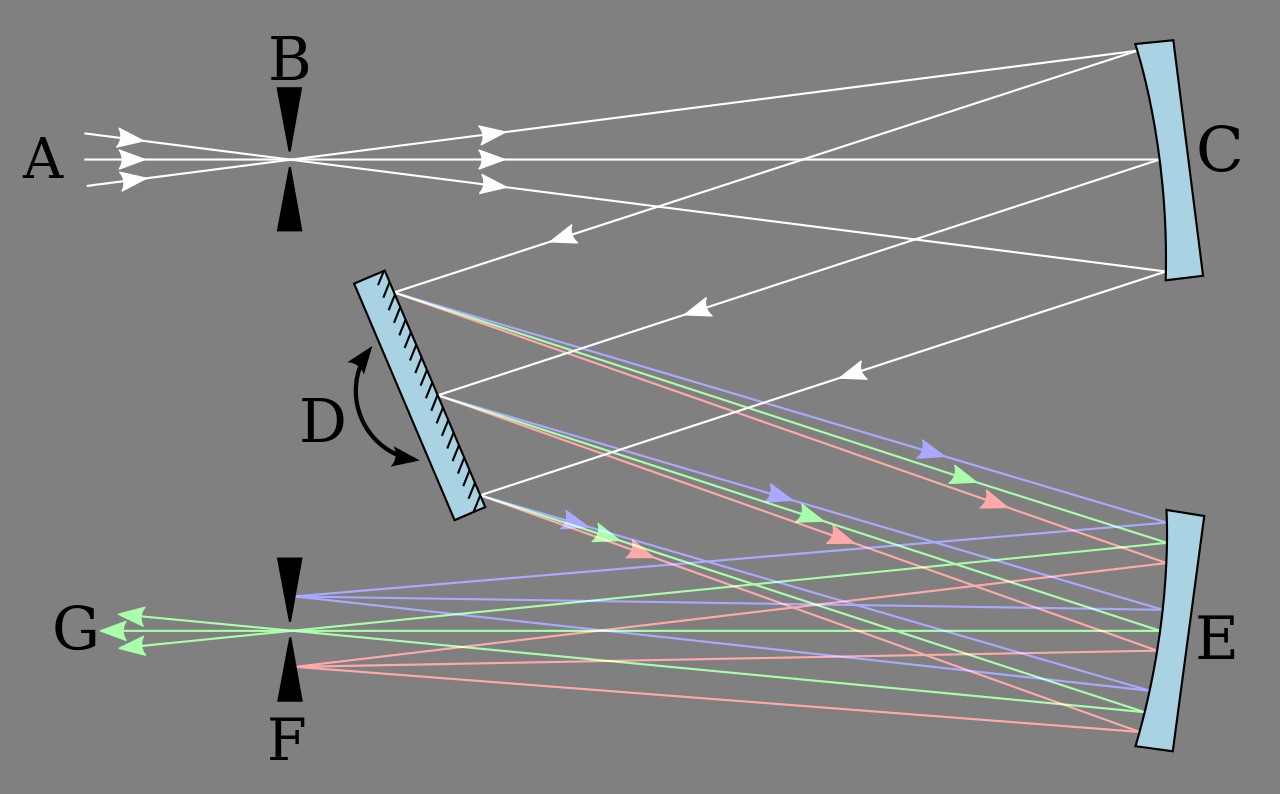
\includegraphics[width=0.4\linewidth]{Imagenes/1280px-Czerny-Turner_Monochromator}
	\caption{Funcionamiento del monocromador. A la salida solo se tiene una longitud de onda. \cite{Czerny-Turney-Conf}}
	\label{fig:1280px-czerny-turnermonochromator}
	
\end{figure}



\section{Tubo fotomultiplicador}
Es un sensor utilizado para poder medir la intensidad luminosa, se le denomina como, PMT, (por sus siglas en inglés, \textit{photomultiplier tube}). Estos sensores, son de alta sensibilidad, son utilizados para medir luz de baja intensidad, o inclusive el conteo de fotones. 
%Los PMts requerían de fuentes de voltajes que iban desde valores de los -1100 volts a los 100 volts, esto para tener diferencias de potenciales en el interior del PMT. Hoy en día existen módulos de PMT que nos permiten ahorrarnos esas fuentes y simplemente conectarlos a $\pm 15$ volts.

Con el monocromador como un sistema para obtener una longitud de onda a la salida y un PMT, como sensor para detectar la intensidad de luminosa a la salida del monocromador, se tienen en principio los elementos para generar espectros.
%tendríamos el principio para construir una relación \textit{intensidad / longitud de onda.} (se modifico.)

\section{Fuentes luminosas.}
Existen varios tipos de fuentes luminosas, como se ha mencionado. Estas pueden tener un espectro de luz continua, de línea, o banda. Una fuente luminosa muy importante para este trabajo es la lámpara de mercurio, que posee un espectro de emisión con líneas perfectamente definidas. En la figura \ref{fig:lamparamercurio} se observan las líneas de emisión que tiene la lámpara HG-01 de la empresa Ocean Optics \cite{Excel2000}. Es útil para calibrar nuestro sistema y con ello, garantizar la relación de \textit{intensidad/longitud de onda.}
\begin{figure}[h]
	\centering
	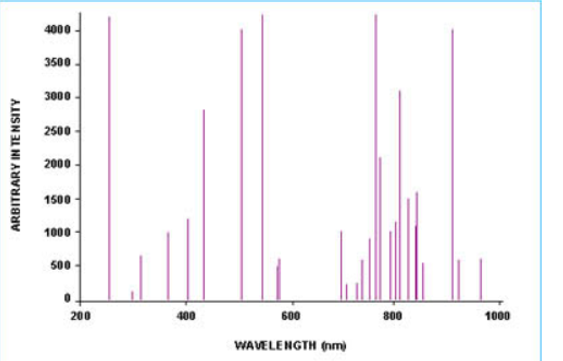
\includegraphics[width=0.7\linewidth]{Imagenes/lamparaMercurio}
	\caption[Espectro de emisión de una lámpara de mercurio a baja presión.]{Espectro de emisión de una lámpara de mercurio a baja presión, la lampara también emite líneas de argón en longitudes de onda mayores a 600 $nm$. \cite{Excel2000}}
	\label{fig:lamparamercurio}
\end{figure}
\section{Propuesta de sistema.}
Con lo mencionado en este capítulo se entiende que se puede construir un espectrómetro automatizado, con un monocromador, un sensor, un motor a pasos y una tarjeta tanto para controlar y adquirir las señales del sistema; como para visualizar el espectro en una interfaz gráfica. 
\section{Antecedentes.}
Como ejemplos de automatización de espectrómetros, en el año 2016, Jie Liu, Zekun Liu y Zhihong Wang utilizaron un encoder magnético AS5048 para la aplicación en el control de la posición de un motor a DC de un espectrómetro portátil. \cite{JieLiu2016}

Más reciente en el año 2017, E. Galli, A. M. Di Giorgio, M. Focardi, E. Pace y G. Micela desarrollaron un software el cual se encarga del control y procesamiento de información del espectrómetro ARIEL (The Atmospheric Remote-sensing Infrared Exoplanet Large-survey. Se implementó un control sobre el AIRS (ARIEL InfraRed Spectrometer). La unidad de control de instrumentos o ICU, por sus siglas en inglés, fue desarrollado con el propósito de que el sistema a bordo fuera suficientemente capaz de implementar las instrucciones funcionales de control y el procesamiento de los datos siendo esto solo la primera parte para este proyecto. \cite{E.GalliA.M.DiGiorgioM.FocardiE.Pace2017}

En países en desarrollo se busca utilizar las herramientas con que se cuenta y aprovecharlas al máximo, al tener presupuestos reducidos, muchas veces nos vemos en la necesidad de reutilizar dispositivos antiguos y darles un nuevo uso o una nueva mejora, utilizando tecnología más reciente. Construir un espectrómetro de alta sensibilidad y resolución utilizando un monocromador es la finalidad de este proyecto, y no es la primera vez que se hace este tipo de trabajos, un ejemplo de ello es la automatización de monocromadores modelo MDR-23, realizado en Rusia, los cuales les servirán para realizar estudios de espectroscopia. \cite{Kraminin2015}

Dentro de la línea de investigación se realizan estudios espectroscópicos de las fuentes luminosas desarrolladas y sobre la interacción de la luz con la materia. Debido al alto costo que conlleva comprar un espectrómetro se decide utilizar los equipos y herramientas con que se cuentan para adaptar un monocromador, que nos servirá para realizar mediciones de espectroscopia.





